%!TEX root = ../Main.tex

%\chapter{Literature review}
%It describes the current status of the wheat genome, genetics and other resources.   

\section{Wheat Breeding}
An overview of how breeding is carried on currently, the different sources of genetic diversity and the relevance of fixing agriculturally important traits. 
\section{Wheat Genetics}
The section describes alleles an the concept of gene, both as a locus in the genome (Quantitative Trait Locus, QTL) and an specific transcript (central dogma of molecular biology). Finally, it discuses traditional Mendelian inheritance and the effect of polyploidy.  Some of this is described in the Yr15 chapter, maybe it is not needed any more here. 




\section{Polyploidy and Wheat}
\label{lit:polyploidy}

A polyploid species contains more than one set of related genomes, that may come from a chromosomal duplication or from an hybridization with a related species. 
\textit{Triticum aestivum} (bread wheat) has gone trough an specialisation event and two major hybridization events. 
Initially, an unknown species first evolved in two different species around 7 million years ago to form the A and B genomes, whose closest known relative are \textit{Triticum urartu} and \textit{Aegelopolis speltoides}. 
As both ancestral wheat were able to cross, at some point around 5.5 million years ago the D genome arouse, \textit{Aegelopolis tauschii}. 
Then, less than 800 thousand years ago the ancient species carrying the  A and B genomes hybridized and formed a tetraploid wheat, \textit{Triticum turgidum} (pasta wheat). 
A final event occurred less than 400 thousand years ago, when pasta wheat hybridized with the carrier of the D genome, leading to bread wheat (Figure \ref{lit:polyploidy}, \citealt{Marcussen2014}).  

\begin{figure}
  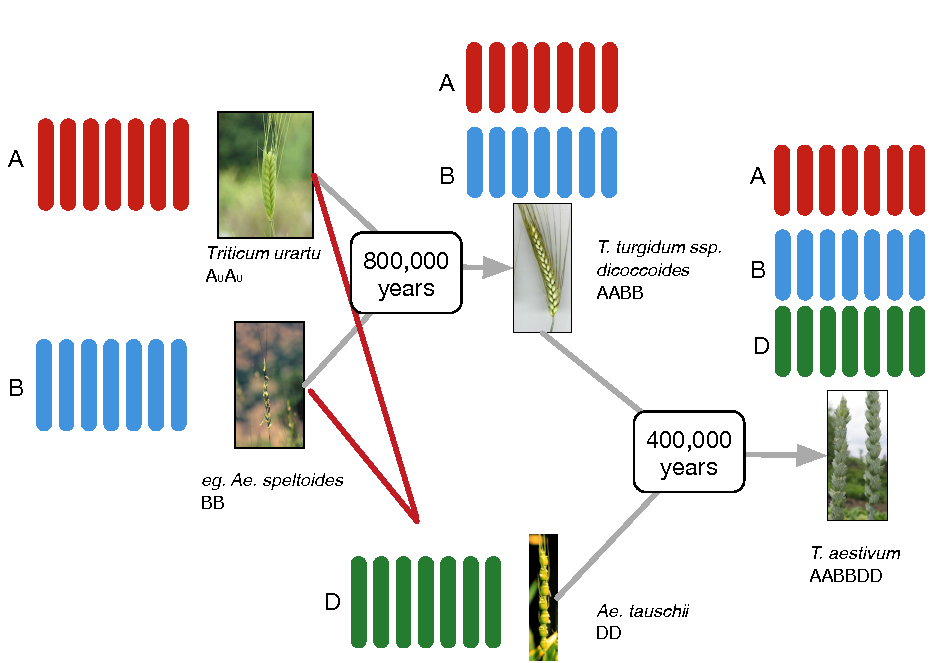
\includegraphics[width=1\textwidth]{LitReview/Figures/WheatPolyplodization.pdf}
  \caption{Hibridizations that lead to bread wheat \textit{T. aestivum}.  }
  \label{fig:lit:polyplody}
\end{figure}
Because bread wheat contains three independent copies of its genome, the expectation is to have three homoeologues for each gene. 

\unsure{Talk about paralogues. }


\section{Wheat Genomics}

A description of the current status of the wheat genome (\citet{Mayer2014}, \citet{Chapman2015}), the different available assemblies and and approaches to sort the scaffolds (Genome Zipper, the various genetic maps).  
\section{Sequencing} 
%The importance of the selection of the library preparation and the sequencing platforms available. A brief summary of RNA-Seq, Exome capture, Whole Genome Shotgun, etc. and on which cases are more suitable for different experiments.  Mention the new technologies developed during the years of the PhD (Ren-Seq, PacBio?)



The Human Genome Project used Sanger sequencing \cite{Lander2001}. This technology is the current gold standard in terms of quality of the sequence. It evolved from electrophoresis gels where the bands represented bases to a fully automated technique. However, the throughput is limited and doing genome wide analysis has prohibitive costs. In the second half of the 2000s high-throughput sequencing technologies emerged which had reduced the cost of sequencing. The main principle of the second-generation sequencing is to produce clusters of clones (i.e. ePCR), fix them in a plate and then add bases with a fluorescent marker. The reaction happens in parallel in millions of clusters at the same time. With each cycle, a picture is taken, showing the fluorescence of each base. Then, image processing algorithms find where in the image the clusters are and the bases are called. At this scale, the volume and complexity of the information is not trivial to manipulate, hence computing is required. 


According to the objectives of the experiment and the quality and volume of the available DNA, the library can be prepared on fragments of different sizes, the classification of the available sequencing for the fragments is the following\cite{Myllykangas2012,Metzker2010,Shendure2008,Hutchison2007}:

\begin{description}
\item[Single end] When the fragments are short, it is possible to just sequence from the 5'-end the read.
\item[Read Pairs] When the sample consists fragments of up to 500bp, it is possible to read the 5' end up to the read length were the quality starts to drop, the molecule can be turned upside down, reverse complemented and sequence backwards. It is not required, but ideally, the fragments sequenced with read pairs should be selected to have an homogenous size. The reads are in opposite orientation relative to each other. 
\item[Overlapping Read Pairs] are a variation to read pairs, where the size of the fragment is shorter than two times the read length. This allow an alignment between the two fragments to get an longer read with the limitations of the instrument.
\item[Mate pairs]  are used to get reads separated at distances between 1kbp and 5kbp. To achieve this, the molecule is circularised and the point were the two ends of the fragment were joint a biotin marker is inserted. Then, the molecule is fragmented again and the fragments containing the biotin are sequenced in the same fashion that read pairs. The resulting reads have the same orientation.
\end{description}


There are several types of experiments that can be analysed with hight throughput sequencing, accordingly, different  protocols for the sample preparation exist. The following is a short list of some of them 

\begin{description}
\item[Whole genome shotgun]  When a sample is prepared for WGS, the DNA is extracted and chopped in fragments  and sequenced. The reads obtained are, in principle, randomly distributed across the whole genome
\item[RNA-Seq].  Instead of sequencing DNA, mRNA is captured and sequenced. The fragments are not amplified in any way, to enable a portrait of the gene expression levels. 
\item[ChIP-SEQ]. Chromatin Immunopresipitation is used to find relationships between proteins and DNA sequence. It is useful to find transcription factors and replication-related proteins.
\item[Amplicon sequencing]. Used primary to do barcoding of species. A known gene is amplified (i.e. 16S) with the intention of characterising the species present in the sample. 
\item[Metagenomic capture] From a mixed sample (soil, root, animal fluids) all the DNA is extracted and sequenced, this gives a snapshot of the microbial community in the sample
\item[RAD-seq] Restriction site associated DNA markers are useful to do population analysis. The technique focus on sequencing regions around restriction sites and the variations around them can be used to genotype individuals. 
\item[Exon capture] The DNA is extracted and baits are used to attract the regions with motif common around exons. This allows to sequence only the genes and regions near them.  
\end{description}


The different sequencing technologies available as of 2013 have different yields, advantages and disadvantages, as described bellow:

\begin{description}
\item[Illumina] Each fragment is amplified using bridge amplification over and over in the same place in the plate to form clusters. After the clusters are formed, a last cycle of amplification is carried on with the bases being added to the template, with the intervention of a polymerase, have a fluorescent marker which make the cluster glow depending on the added base. It adds one base per cycle.     With a read length between 75bp and 250bp is currently the most widely adopted platform. The As a de facto standard, many tools exist to cope bioinformatically with the biases of the machine.  The run takes 4 or 9 days, depending on days, depending if one or two reads are generated for each fragment. It produces up to 35 gigabases per run. 

\item[SOLiD] The preparation of the fragments is similar to Illumina, however, when adding the bases they are added in pairs. This technique is called sequencing by ligation as it use a DNA Ligase, as opposed to a polymerase, to determine the transition between bases. The resulting sequence is not in base space, but in colour space, which represents the transition state between bases. This technique is robust for finding SNPs when you have a good reference where to align the reads. However, the number of tools available and the research done to analyse sequences in colour space is low compared to the tools using base space. The runs take between one and two weeks to complete, with a yield of up to 50 gig abases per run. The read length can be up to 50 bases

\item[Roche/454] The fragments are cloned in beads, which then fall in wells in the slide. The sequencing is done by adding nucleotides in a determined order. The next nucleotides to be added in the reaction contain a fluorescent marker. The bases are not added one by one, but all the bases that are the same are added together. The amount of glow on each well can tell how many times a base is added. As the glow is not a discrete number, when a long homopolymer appear (above 5 bases) the likelihood of having a wrong count of the homopolymer is increased.  The average read length varies between 300 and 700bp. A run usually takes half a day, but it only yleds 0.45 gigabases. The cost of the reagents is relatively expensive, but if the experiment requires longer reads it is a good option. 

\item[PacBio] Opposed to all the previous technologies, Pacific Biosciences has developed a sequencing technology where the molecules doesn't need to be PCR amplified before the sequencing. The glass slide used contains wells with a depth of 100nm where a polymerase lays at the bottom. The nucleotides to be added have a fluorescent marked that is freed when the polymerase adds the nucleotide, releasing a light signal, which then can be captured from the bottom of the glass. The error rate for this technology is still high (about 10\% of the bases are miscalled), however reading several times the same molecule reduce the error rate. The main advantage is that the reads can be over 1kbp. 

\item[OpGen] Additionally, high-througput optical mapping technologies, like OpGen, are becoming accessible.  The maps are done by fixing single molecules of DNA are held on a slide. Then,  restriction enzimes targeted to specific digestion sites cut the fragment and fluorescent markers are added to the ends of the fragments. Finally, the fragments are visualised and the size of the molecules is measured by the distance between fluorescent points in the slide. This is done with several fragments at the same time. Then, the distances between restriction sizes can be compared across all the fragments to generate a consensus. Finally, if you have contigs from other technologies, it is possible to complement the information and get better assemblies. Even without the contigs, the data can be used to compare translocations within strains of different bacteria or homologous species at a chromosome level. 

\item[ION Torrent] (Do some research on newer sequencing things)

\end{description}

\section{Sequence analysis}
This section discusses the criteria to decide analysis done after sequencing, when to do re-alignments or \textit{de novo} assemblies, how to do SNP calling in diploid and polyploid organisims and the bulk frequency ratios.  



DNA sequence alone is not alone to enough to understand the biology behind, a context is required. There are databases like Ensembl and NCBI that act as repositories of the known public sequences. 

From the computational point of view, the problem can be viewed as a string matching. The Smith-Waterman\cite{Smith1981} and Needleman-Wunsch\cite{Needleman1970} algorithms are the gold standard interns of accuracy looking for similarity between sequences. However, the execution time for both of them is prohibitive to run in massive databases. The algorithm execution time is O(mn), as it requires calculating a matrix of size $mn$ where $m$ is the target sequence and $n$ is the query sequence.  To scale this to a manageable problem algorithms like BLAST index the references and use heuristics to make the search more manageable, with some penalty in the accuracy. This alignments tools are useful for long stretches of DNA (like cDNA or contigs)\cite{Altschul1990}.

TODO: List of global aligners
-BLAST
-BLAT
-Exonerate
-nucmer


When looking at a protein level, where the sequences may be only loosely similar, Hidden Markov Models (HMM) are used to search for protein families. This can be useful to annotate putative proteins and their functions. HMMs require a training dataset, where proteins are previously annotated and the reference is a model encoding the characteristics of a family, with associated probabilities. Hence, this technique is something between a sequences aligner and a classifier\cite{Eddy2004}. 

When analysing high-throughput sequencing, having millions of short sequences make unfeasible to try to align the data to every possible reference. However, one can take in advantage the fact that you know which organism you are looking for and, if available, use a genomic reference. For this, tools like MAQ, BWA, Bowtie, among others, provide indexed search.  Once you have your reads aligned to a reference you can do more analysis, depending on the biological question being asked and the type of sequencing carried on.  Fortunately, most of the Short-Read sequence alignment produce similar outputs and the SAM format is becoming a de facto standard. This is allowing to make more modularised downstream analysis where you can test different aligners with different settings and pick the algorithm that better fits your experiment\cite{Liu2012,Li2009,Li2009a}. 

\subsection{Ambiguity Codes}
\label{lit:ambiguity}
Make a table with the ambiguity codes and why they are useful. 




\subsection{RNA-Seq}
\label{lit:RNASeq}

One way to narrow down which genes are involved in certain trait or response to the environment is to focus on studying only the expressed genes. One of the techniques involving high-throughput sequencing is RNA-Seq. This technique captures the messenger RNA in the tissue being studied and sequenced. The premise is that you will find a gene more expressed if it is being used by the organism. Some proteins with a vital role for the cell are always expressed (i.e. RuBisCO for carbon fixation in plants\cite{CooperGM2000}). On the simplest of the experiments you would need two datasets to compare, one with the gene being looked expressed and one where it is not. The expression can come from different environmental conditions, development stage or different genotypes.\cite{Mortazavi2008} 

Depending on how much \textit{a priori} information of the analysed organism is available different bioinformatic approaches can be used.
\begin{description}
\item[Transcriptome alignment] The reads are aligned to a database of known cDNA. Ideally, alternative splicing sequences are available, so a simple alignment should work (i.e. BWA, bowtie). 
\item[Genomic alignment] The reads are aligned to the genome. The splice junctions, introns and axons need to be accounted, so simple alignment doesn't work. Regular alignments are used, but the reads may be trimmed at fixed sizes to allow discontinuous alignments using regular tools (i.e. Stampy, tophat/cufflinkns)
\item[\textit{De Novo} transcriptome assembly] If a reference of the organism is not available, it is possible to generate a draft transcriptome with the RNA-Seq reads with traditional assemblers (velvet, abyss) or with specialised assembler tools like Trinity. 
\end{description}

Once you have the alignments it is possible to evaluate the relative expression of the genes in the sample calculating the Reads per Kilobase per Million mapped reads (RPKM) or the Transcripts per Million (TPM). This normalises the expression by the amount of sequenced data and can be used to find which genes change in expression volume across different samples.   
%TODO: Write more details of RPKM vs TPM

%\subsection{Bulk Frequency Ratios}
%\label{sub:lrBFR}
%The tools mentioned above are designed with diploids in mind and tested in model organisms like human, mouse, arabidopsis. Besides, using the RPKMs only gives you an idea of the amount of expression. However, the some experiments are intended to characterise particular variations that provide certain phenotype. When analysing polyploid organisms, like hexaploid wheat, up to six variations of the same gene can be present, but only one of them is actually providing the phenotype being studied. To be able to find  this variants it is possible to calculate the Bulk Frequency Ratios (BFR). 



% The BFR helps reduce the noise generated by differential expression of homoeologous genes and accounts for the presence of alternative bases at any given position. A closely linked SNP to the R-gene should generate a very high BFR since the resistant bulk will carry exclusively plants with the resistant allele, whereas the susceptible bulk should be devoid of any plants carrying the resistant allele. As one moves further away from the R-gene, recombination events occur between the gene and the candidate SNPs decreasing the BFR.

\section{Wheat specific resources resources}
\label{lit:wheatResourcers}
Gene models
-UniGene
-UCW Gene models
-Gene annotation IWGSC
-Gene annotation TGACv1

Genetic maps
-Wang
-Chapman/PopSeq (is the same populaiton, improved)

Markers
-90k
-820k
-MASwheat/SRR

Portal
-CeralsDB
-MASWheat
-Ensembl
-Wheat-expression

Assemblies
-Chapman
-IWGSC
-TGACv1
-NRGene (unpublished?)
-454 Liverpool

A compilation of the currently available resource for whet genetics and genomics. MAS wheat, CeralsDB, Ensembl, etc.  

\section{Programming languages}
Why Ruby and javascript?
-Ruby
-BioRuby
-JavaScript
-BioJS
-Rails. 
-SQL

-lamda functions
-functions/methods

-object orientation
-hashes
-design patterns
 -Containers, as in AWT. 

 \label{lit:patterns}